\documentclass[border=1mm]{standalone}
\usepackage{amsfonts,tikz,tikz-layers}
\usetikzlibrary{fadings,quotes, shapes,calc,decorations.markings}
\usetikzlibrary{patterns}
\usetikzlibrary{shadows.blur}
\usetikzlibrary{shapes,shapes.geometric,positioning, arrows, arrows.meta}
\usetikzlibrary{backgrounds}

\begin{document}
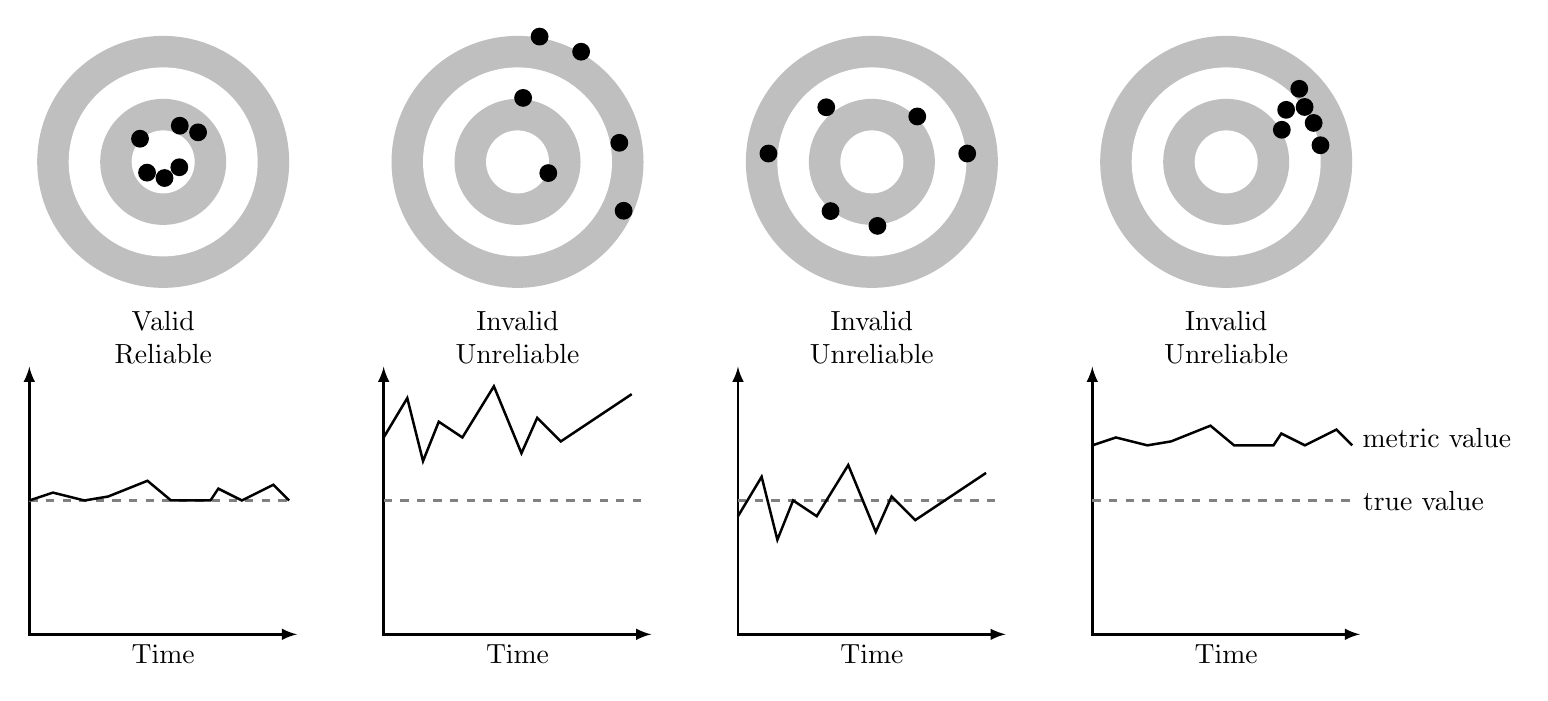
\begin{tikzpicture}[line width=.9pt]
%Valid Reliable
% Circles
\node[circle, fill=lightgray, minimum size=4*.8cm] (A) {};
\node[circle, fill=white, minimum size=3*.8cm] (A1) {};
\node[circle, fill=lightgray, minimum size=2*.8cm] (A2) {};
\node[circle, fill=white, minimum size=1*.8cm] (A3) {};

\node[circle, fill=black, scale=.24mm, shift={(.3,-.1)}] at (A3.center) {};
\node[circle, fill=black, scale=.24mm, shift={(-.3,-.2)}] at (A3.center) {};
\node[circle, fill=black, scale=.24mm, shift={(0.025,-.3)}] at (A3.center) {};
\node[circle, fill=black, scale=.24mm, shift={(0,0)}] at (A3.90+45) {};
\node[circle, fill=black, scale=.24mm, shift={(0.1,0.1)}] at (A3.70) {};
\node[circle, fill=black, scale=.24mm, shift={(0.15,0.2)}] at (A3.35) {};
% Text node
\node[align=center, below=0.15cm of A] {Valid\\Reliable};
% Axis graph
\draw[black,latex-latex] (1.7,-6)-- node[below, black]{Time} ++(-3.4,0)--+(0,3.4);
\draw[gray, dashed, line width=1.2pt] (-1.7,-4.3)--+(3.3,0);
\draw[black] (-1.7,-4.3)--++(.3,.1)--++(.4,-.1)--++(.3,.05)--++(.5,.2)--++(.3,-.25)--++(.5,0)--++(.1,.15)--++(.3,-.15)--++(.4,.2)--+(.2,-.2);
% Invalid Unreliable
\begin{scope}[xshift=4.5cm]
% Circles
\node[circle, fill=lightgray, minimum size=4*.8cm] (A) {};
\node[circle, fill=white, minimum size=3*.8cm] (A1) {};
\node[circle, fill=lightgray, minimum size=2*.8cm] (A2) {};
\node[circle, fill=white, minimum size=1*.8cm] (A3) {};

\node[circle, fill=black, scale=.24mm, shift={(0,0)}] at (A2.85) {};
\node[circle, fill=black, scale=.24mm, shift={(0,0)}] at (A3.-20) {};
\node[circle, fill=black, scale=.24mm, shift={(0,0)}] at (A.80) {};
\node[circle, fill=black, scale=.24mm, shift={(0,0)}] at (A.60) {};
\node[circle, fill=black, scale=.24mm, shift={(-0.25,-0.1)}] at (A.-20) {};
\node[circle, fill=black, scale=.24mm, shift={(0.12,0.2)}] at (A1.5) {};
% Text node
\node[align=center, below=0.15cm of A] {Invalid\\Unreliable};
% Axis graph
\draw[black,latex-latex] (1.7,-6)-- node[below, black]{Time} ++(-3.4,0)--+(0,3.4);
\draw[gray, dashed, line width=1.2pt] (-1.7,-4.3)--+(3.3,0);
\draw[black] (-1.7,-3.5)--++(.3,.5)--++(.2,-.8)--++(.2,.5)--++(.3,-.2)--++(.4,.65)--++(.35,-.85)--++(.2,.45)--++(.3,-.3)--++(.9,.6);
\end{scope}
%----------------------Valid Unreliable ---------------------------------
\begin{scope}[xshift=9cm]
% Circles
\node[circle, fill=lightgray, minimum size=4*.8cm] (A) {};
\node[circle, fill=white, minimum size=3*.8cm] (A1) {};
\node[circle, fill=lightgray, minimum size=2*.8cm] (A2) {};
\node[circle, fill=white, minimum size=1*.8cm] (A3) {};

\node[circle, fill=black, scale=.24mm, shift={(-.15,0)}] at (A1.175) {};
\node[circle, fill=black, scale=.24mm, shift={(-.08,.1)}] at (A2.90+40) {};
\node[circle, fill=black, scale=.24mm, shift={(0,0)}] at (A2.45) {};
\node[circle, fill=black, scale=.24mm, shift={(0,0)}] at (A2.-85) {};
\node[circle, fill=black, scale=.24mm, shift={(0,0)}] at (A2.-130) {};
\node[circle, fill=black, scale=.24mm, shift={(0,0)}] at (A1.5) {};
% Text node
\node[align=center, below=0.15cm of A] {Invalid\\Unreliable};
% Axis graph
\draw[black,latex-latex] (1.7,-6)-- node[below, black]{Time} ++(-3.4,0)--+(0,3.4);
\draw[gray, dashed, line width=1.2pt] (-1.7,-4.3)--+(3.3,0);
\draw[black] (-1.7,-4.5)--++(.3,.5)--++(.2,-.8)--++(.2,.5)--++(.3,-.2)--++(.4,.65)--++(.35,-.85)--++(.2,.45)--++(.3,-.3)--++(.9,.6);
\end{scope}
%Invalid Reliable
\begin{scope}[xshift=13.5cm]
% Circles
\node[circle, fill=lightgray, minimum size=4*.8cm] (A) {};
\node[circle, fill=white, minimum size=3*.8cm] (A1) {};
\node[circle, fill=lightgray, minimum size=2*.8cm] (A2) {};
\node[circle, fill=white, minimum size=1*.8cm] (A3) {};

\node[circle, fill=black, scale=.24mm, shift={(.2,.2)}] at (A2.40) {};
\node[circle, fill=black, scale=.24mm, shift={(0.1,0.1)}] at (A1.45) {};
\node[circle, fill=black, scale=.24mm, shift={(0,0)}] at (A1.35) {};
\node[circle, fill=black, scale=.24mm, shift={(0,0)}] at (A1.24) {};
\node[circle, fill=black, scale=.24mm, shift={(0,0)}] at (A1.10) {};
\node[circle, fill=black, scale=.24mm, shift={(0,0)}] at (A2.30) {};
% Text node
\node[align=center, below=0.15cm of A] {Invalid\\Unreliable};
% Axis graph
\draw[black,latex-latex] (1.7,-6)-- node[below, black]{Time} ++(-3.4,0)--+(0,3.4);
\draw[gray, dashed, line width=1.2pt] (-1.7,-4.3)-- node[pos=1,right,black] {true value} +(3.3,0);
\draw[black] (-1.7,-3.6)--++(.3,.1)--++(.4,-.1)--++(.3,.05)--++(.5,.2)--++(.3,-.25)--++(.5,0)--++(.1,.15)--++(.3,-.15)--++(.4,.2)--node[pos=1,right,black,yshift=.1cm] {metric value}+(.2,-.2);
\end{scope}

\end{tikzpicture}

\end{document}
